\documentclass{bioinfo}
\copyrightyear{2022} \pubyear{2022}



% tightlist command for lists without linebreak
\providecommand{\tightlist}{%
  \setlength{\itemsep}{0pt}\setlength{\parskip}{0pt}}




% hyperref makes the margins screwy.
% https://groups.google.com/forum/#!topic/latexusersgroup/4W_SwGk6zx4
% http://ansuz.sooke.bc.ca/software/latex-tricks.php
% \usepackage[colorlinks=true, allcolors=blue]{hyperref}

\access{Advance Access Publication Date:   }
\appnotes{Application Note}

\begin{document}


\firstpage{1}

\subtitle{Genome analysis}

\title[Clustering Bird Species]{Clustering Size Measurements of Extinct
and Extant Bird Species}

\author[FirstAuthorLastName \textit{et~al}.]{
Fiel Dimayacyac\,\textsuperscript{1}
}

\address{
\textsuperscript{1}University of British Columbia, Bioinformatics,
Vancouver, British Columbia\\
}

\corresp{}

\history{Received on XXX; revised on XXX; accepted on XXX}

\editor{Associate Editor: XXX}

\abstract{
\textbf{Motivation:} Identify if extinct and extant birds cluster
according to order, extinction status, or flightlessness using size
measurements.\\
\textbf{Results:} This analysis found that bird size data minimized
total within sum of squares with a k means of seven, but that bird size
measurements did not cluster according to extinction status or
flightlessness. Some clustered according to taxonomic relationship.\\
\textbf{Availability:} All scripts, data, and manuscript files are
freely available on the web at the Open Science Foundation website.\\
\textbf{Contact:}fieldimayacyac@gmail.com\\
\textbf{Supplementary information:} Supplementary data are available on
the Open Science Foundation website.}

\maketitle

\section{Introduction}

In this study I reanalyze the paper by \citet{fromm_big_2021} wherein
the authors aggregated body size measurements, flightlessness, order,
and habitat of 9000 bird species with a focus on identifying size trends
between extant species and species driven to extinction by human
intervention. \citet{fromm_big_2021} found a significant difference
between extinct and extant birds in overall body size and other factors,
concluding that species driven to extinction tended to be larger,
flightless, and island-dwelling.

My aim is to see if those trends hold up in the body size data itself;
i.e., can an unsupervised learning approach naively discover these same
trends. Specifically, I use k-means clustering as implemented in the
tidymodels R package \citep{kuhn_tidymodels_2020}.

\section{Results}

Before performing k-means clustering, I first cleaned the data, and then
selected variables to use later. I found that much of the data was
unavailable, so I chose two bone measurements with the most overlapping
available data points that included both extinct and extant species.
These bone measurements being for humerus and tarsometatarsus.

Following data filtering I then visualized the remaining data to see if
there were any obvious trends across extinction status, flightlessness,
or order. Axes were log-normalized for inter-specific comparisons. No
evident trends were visible previous to clustering (Figure 1).

\begin{figure}
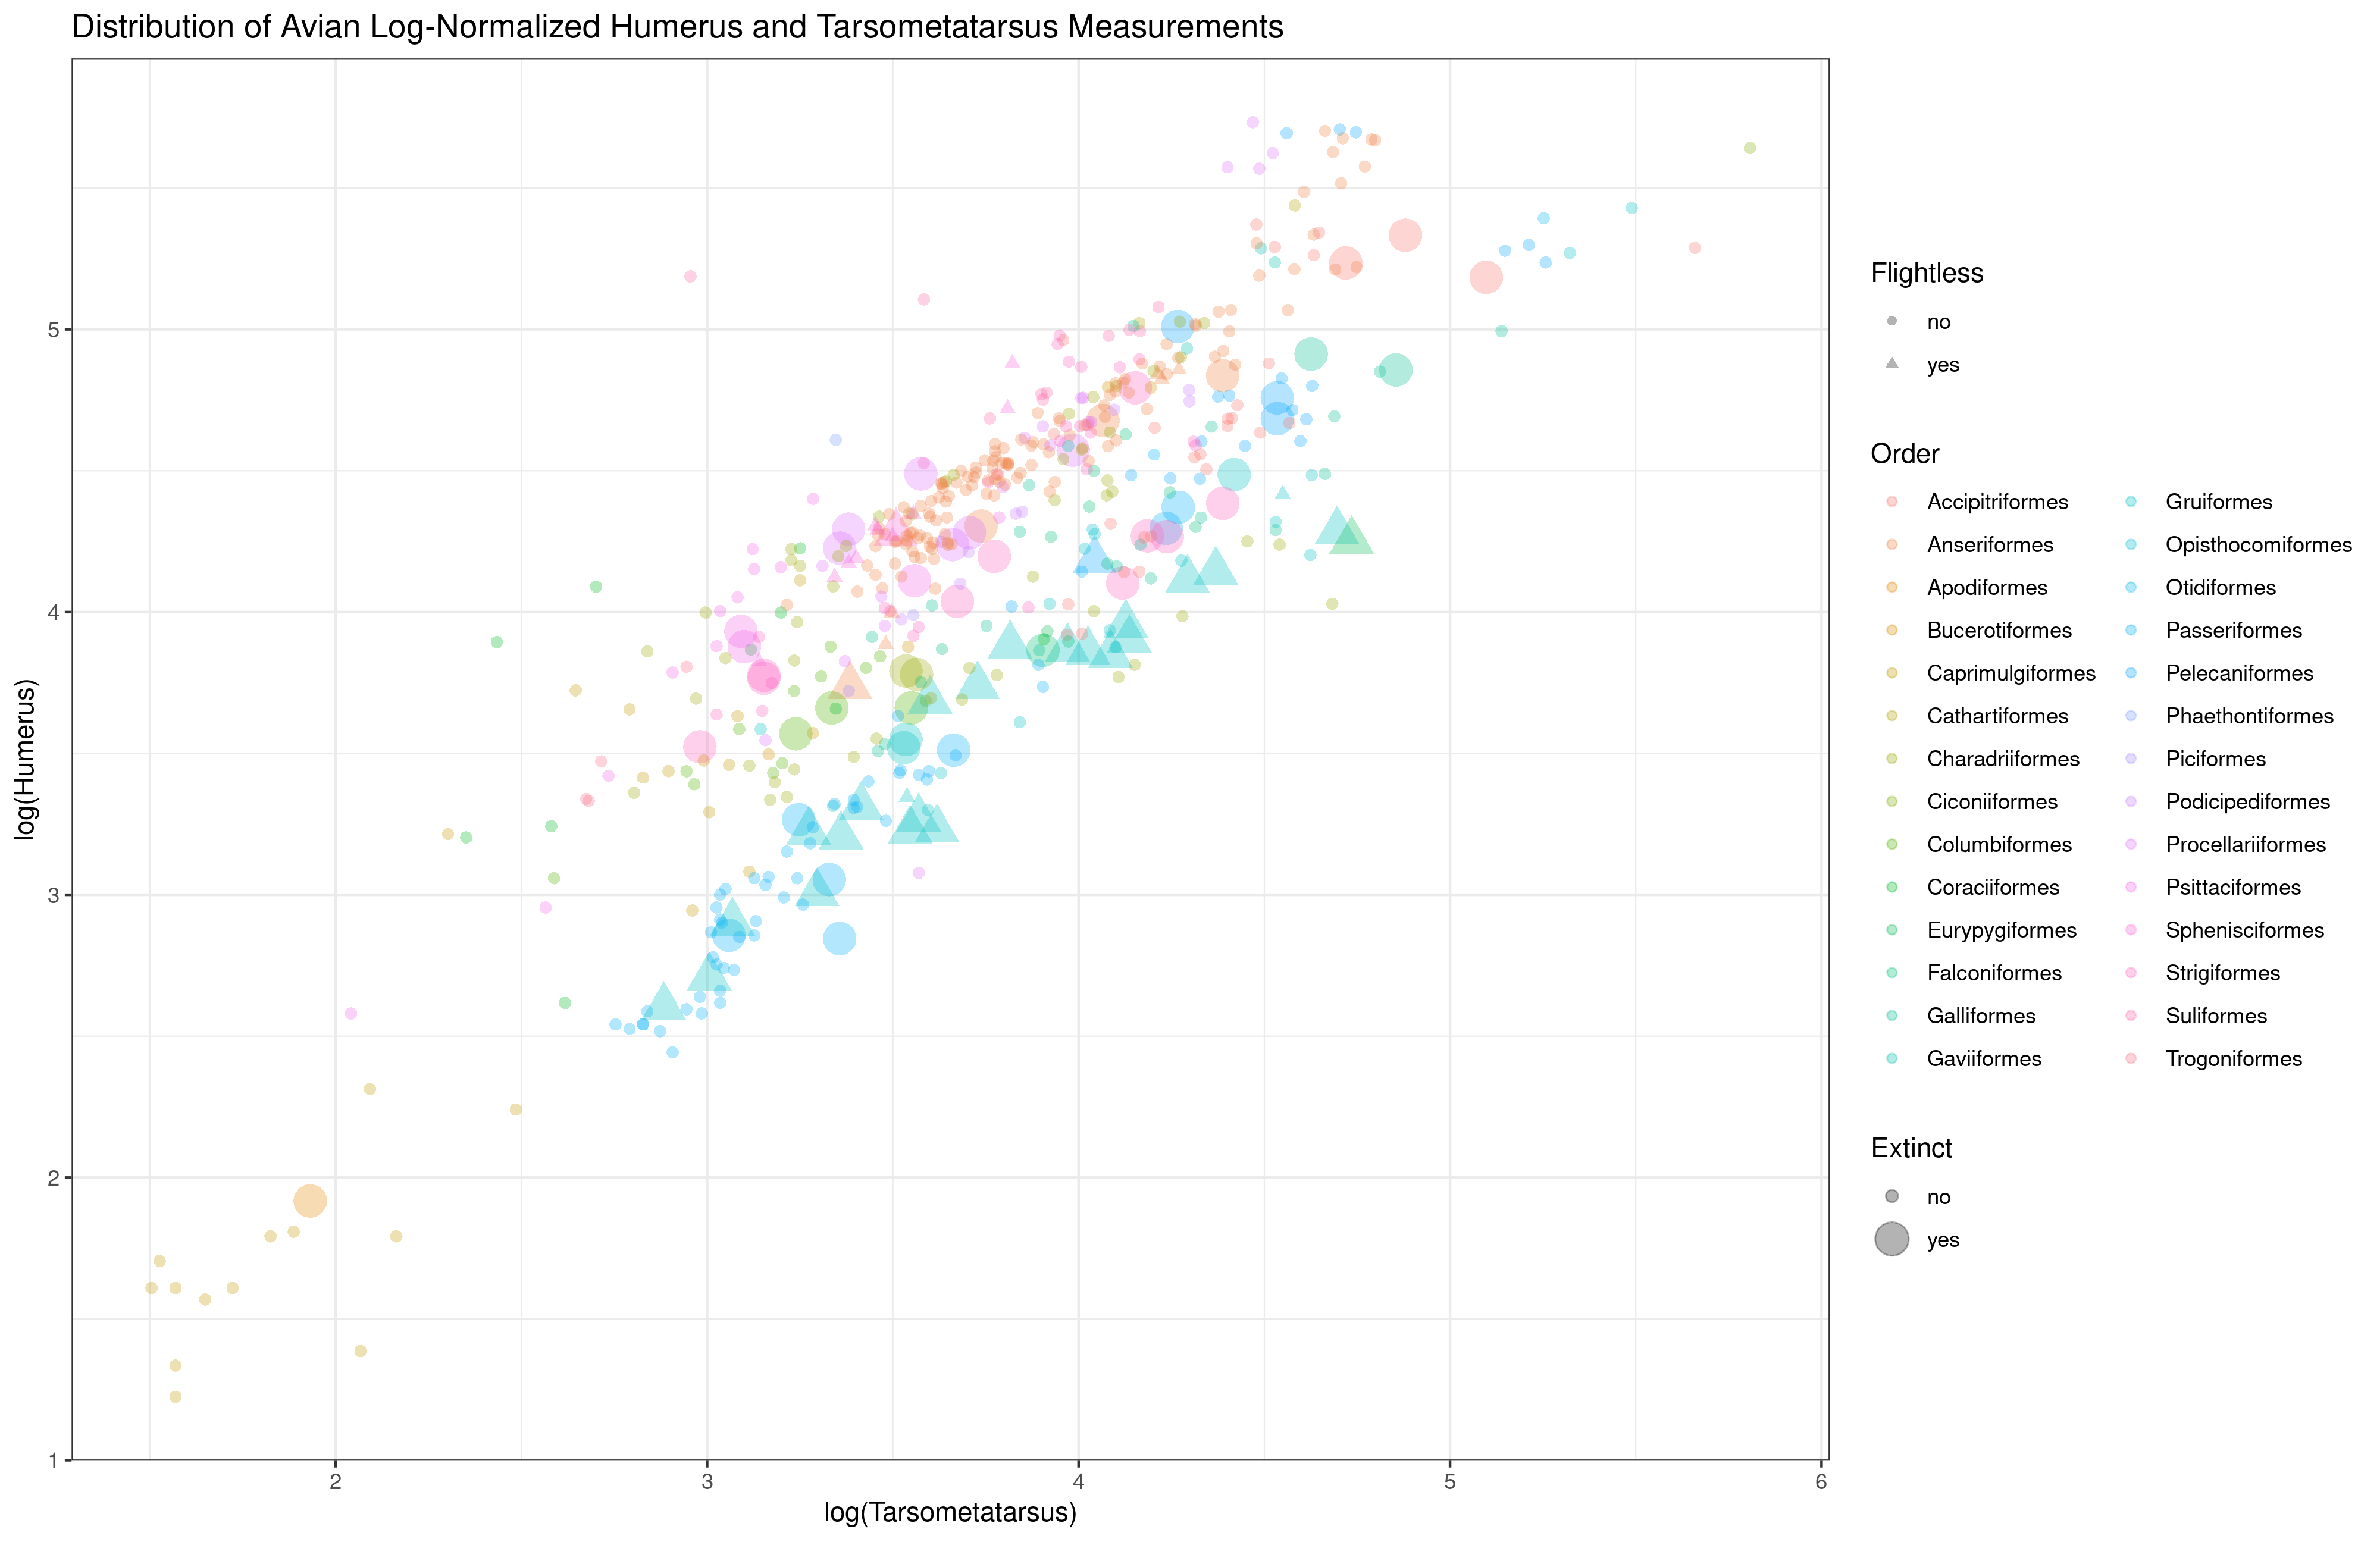
\includegraphics[width=1\linewidth]{../outputs/pre_cluster_plot} \caption{Distribution of size measurements for extinct and extant bird species with flightlessness, Order, and extinction status. Tarsometatarsus measurements are on the x-axis and Humerus measurements are on the y-axis}\label{fig:figure1}
\end{figure}

To identify the optimal number of k-means to describe the patterns in
the data, I then performed k-means analysis, varying the k value from
one to ten (Figure 2).

\begin{figure}
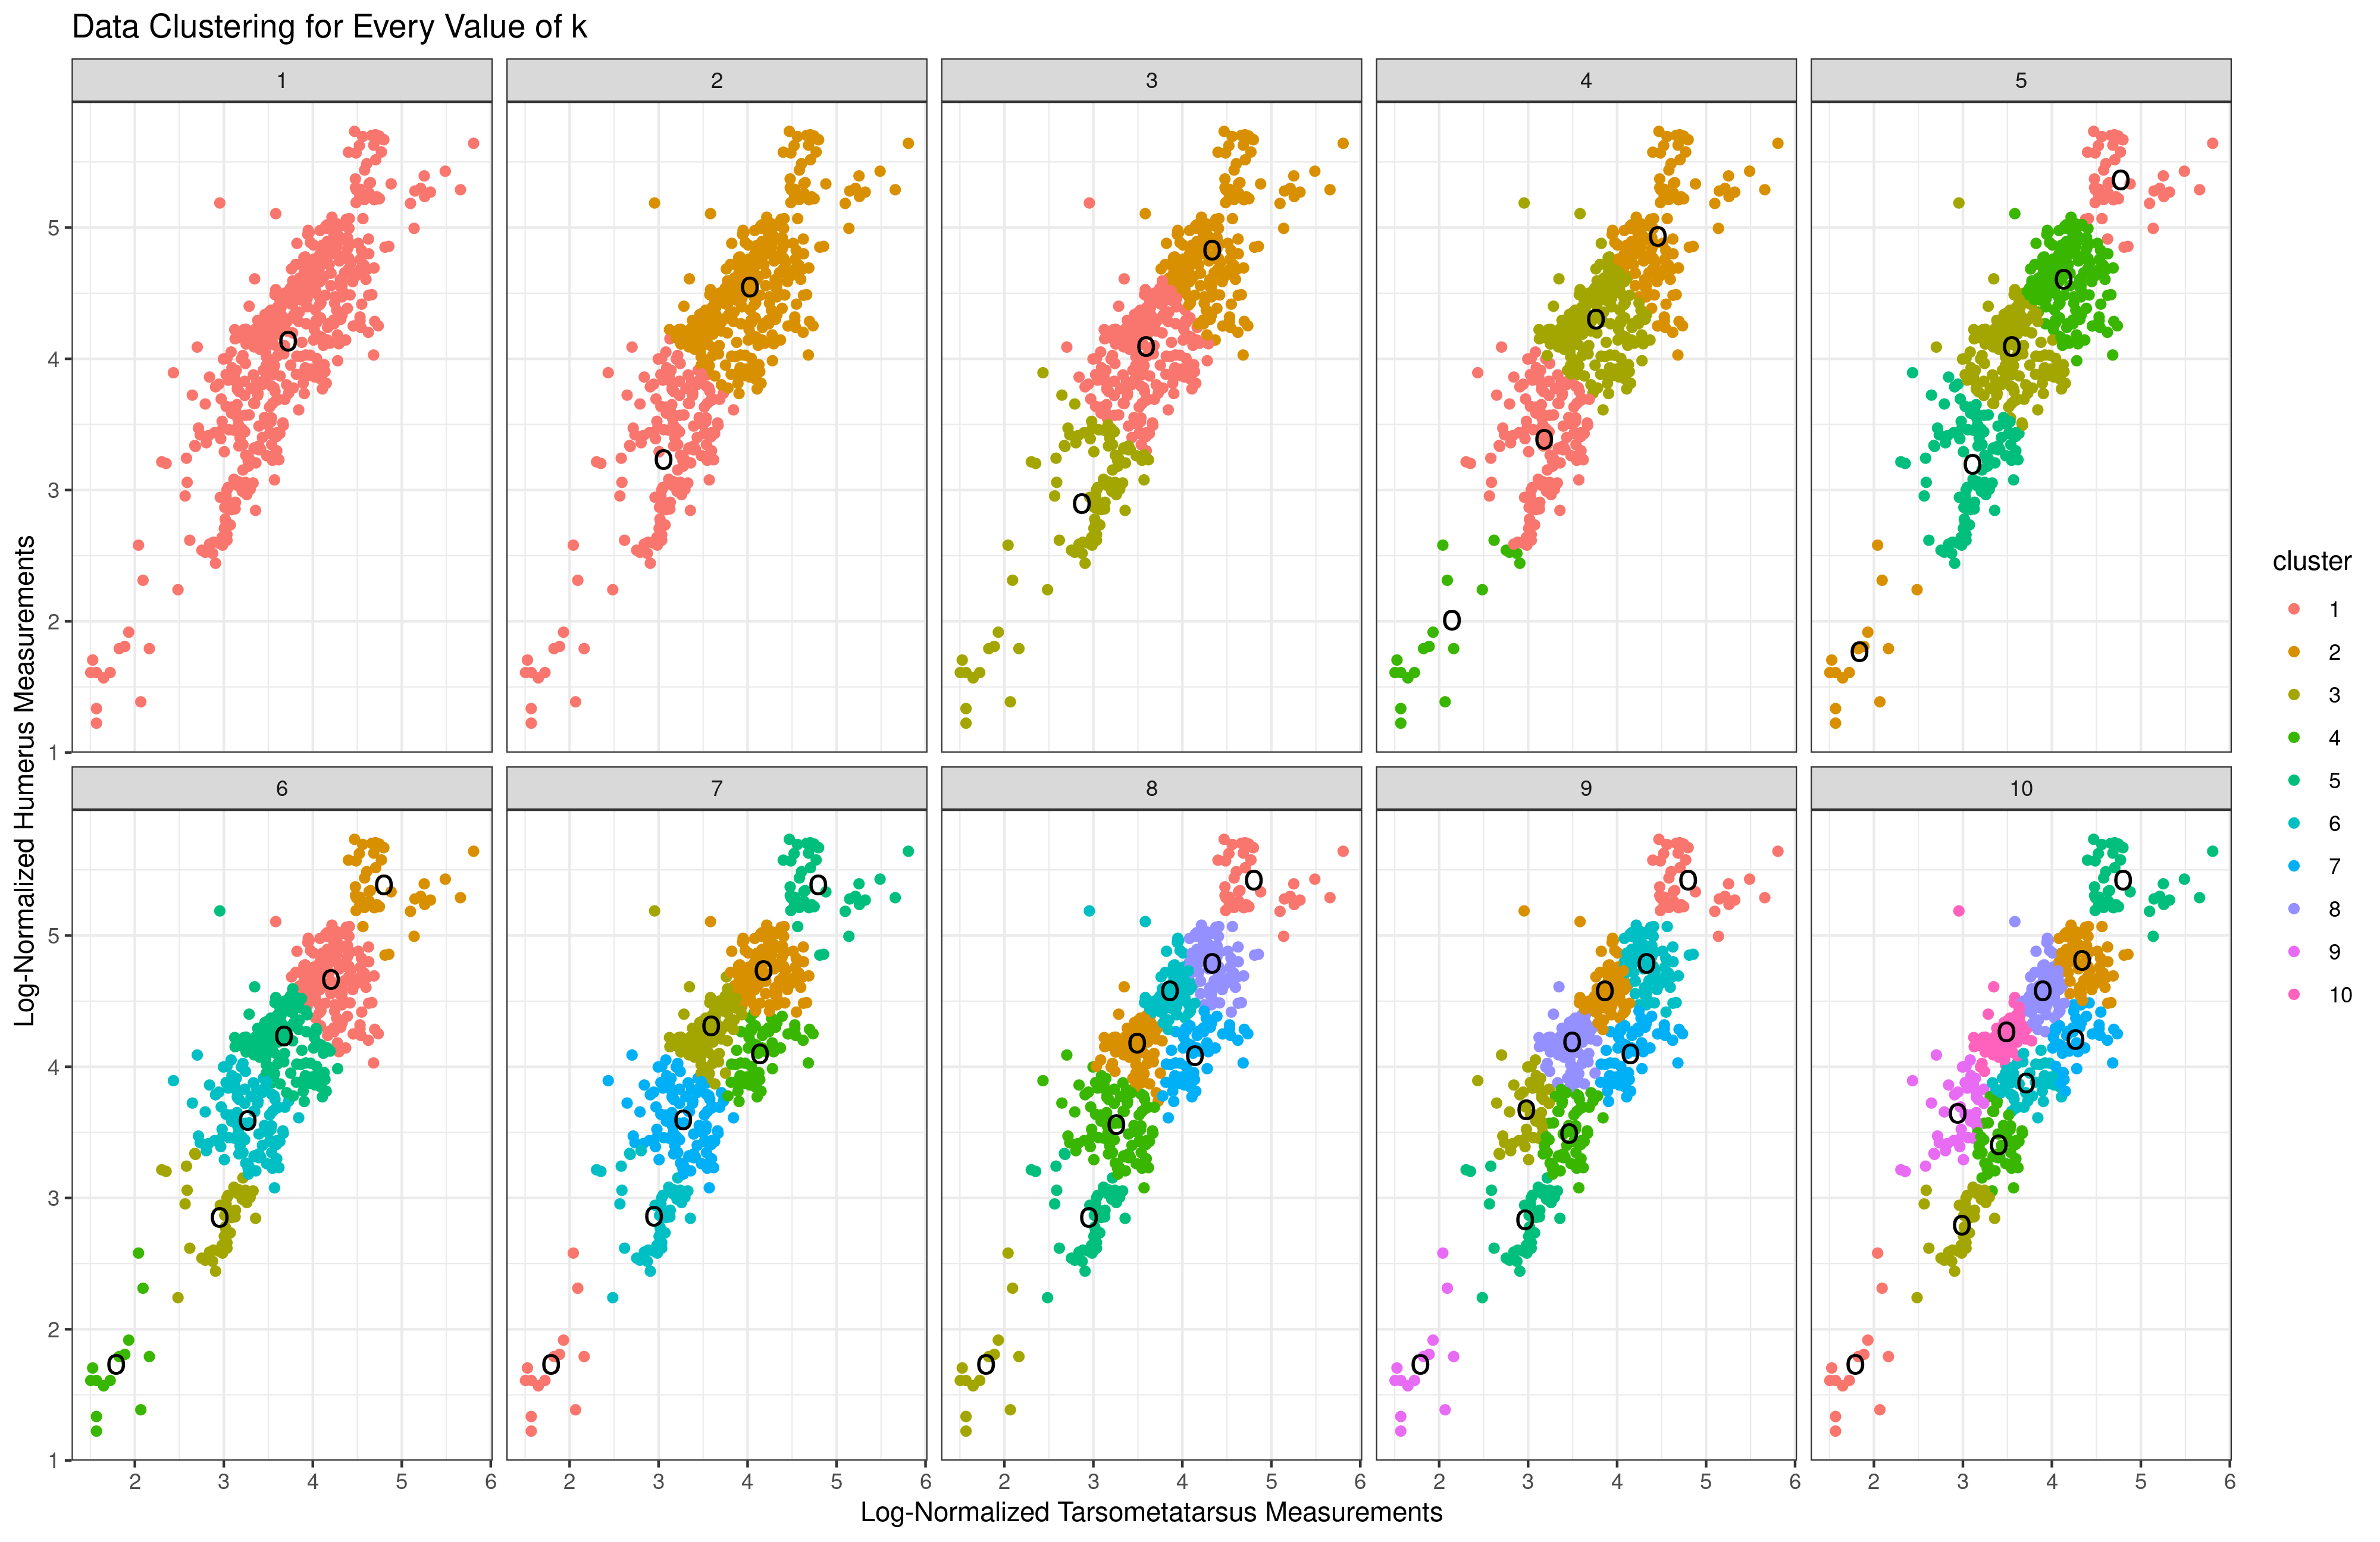
\includegraphics[width=1\linewidth]{../outputs/centered_clusters} \caption{Clustered size measurement data with varying values of k. Circles represent cluster centers}\label{fig:figure2}
\end{figure}

To quantify how optimal each k-means value was, I calculated the total
within sum of squares for each value k for the model. The lowest value k
that minimized the total within sum of squares was seven (Figure 3).

\begin{figure}
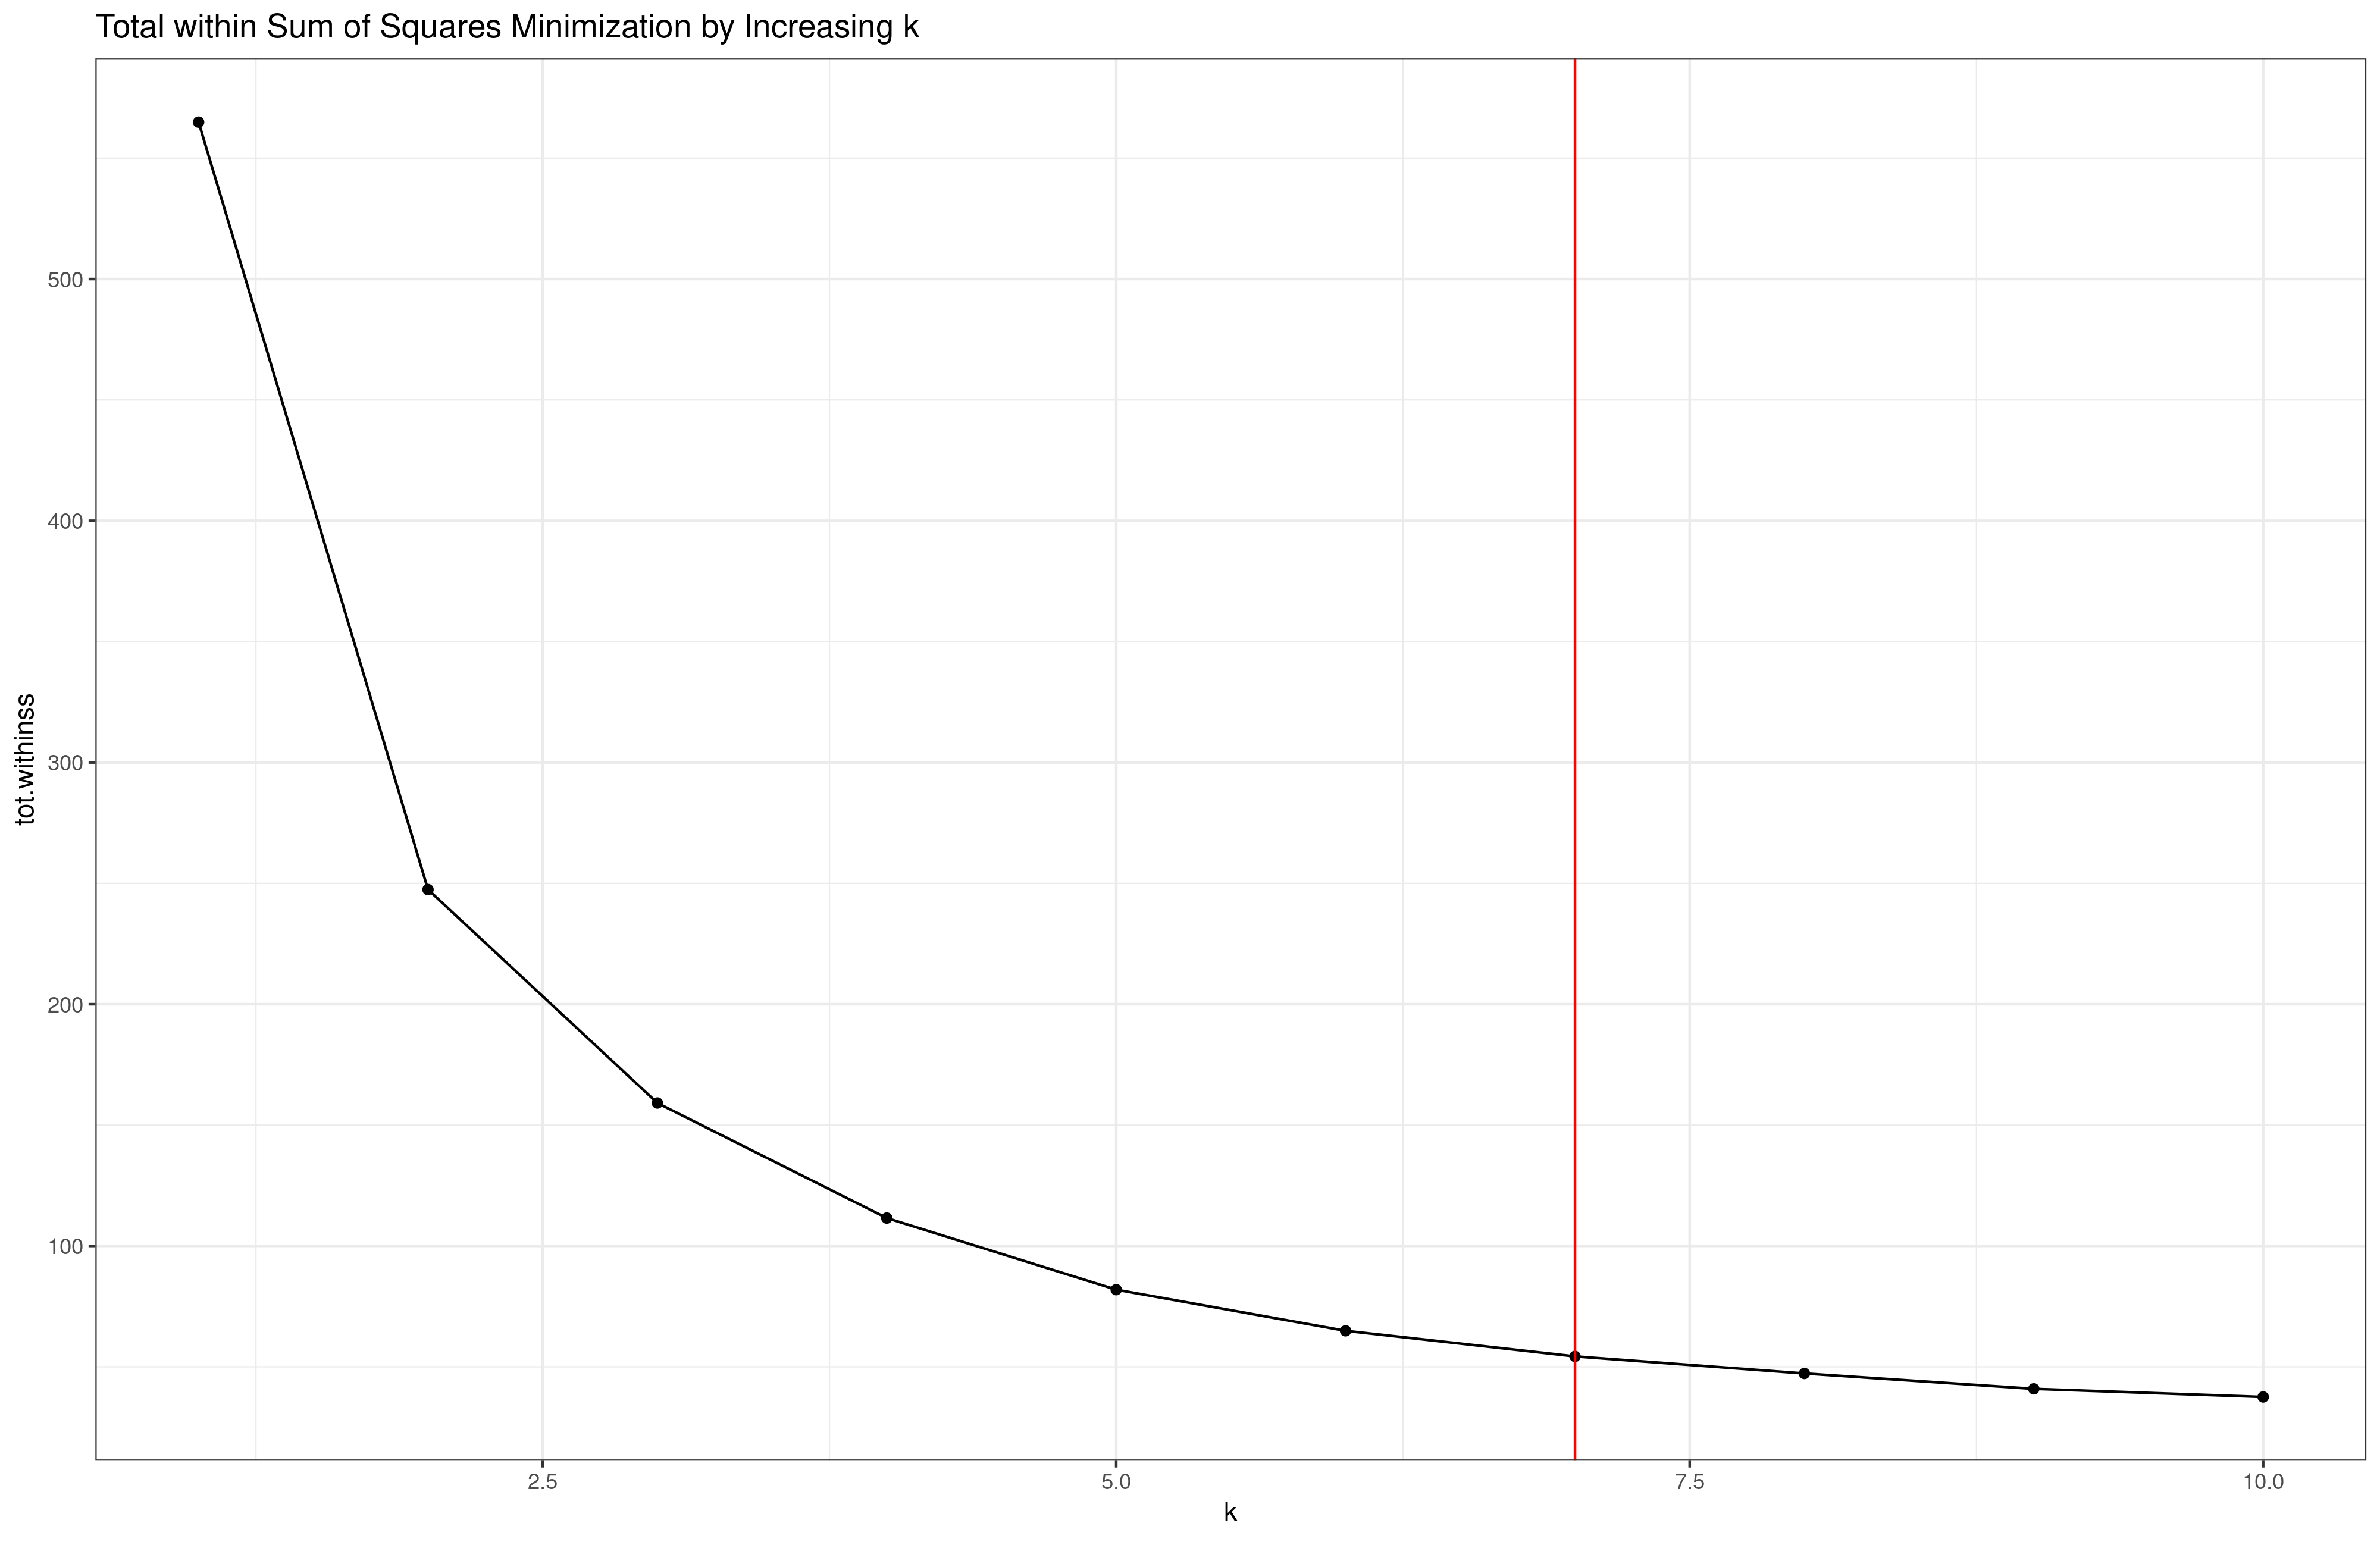
\includegraphics[width=1\linewidth]{../outputs/tot.withinss_minimization} \caption{Total within sum of squares for varying k values. The red line intersects at a k of seven}\label{fig:figure3}
\end{figure}

Finally, I plotted the clusters with a k of seven overlaid onto Figure 1
to identify if there were any trends within the clusters. No noticeable
trends were evident in the data (Figure 4).

\begin{figure}
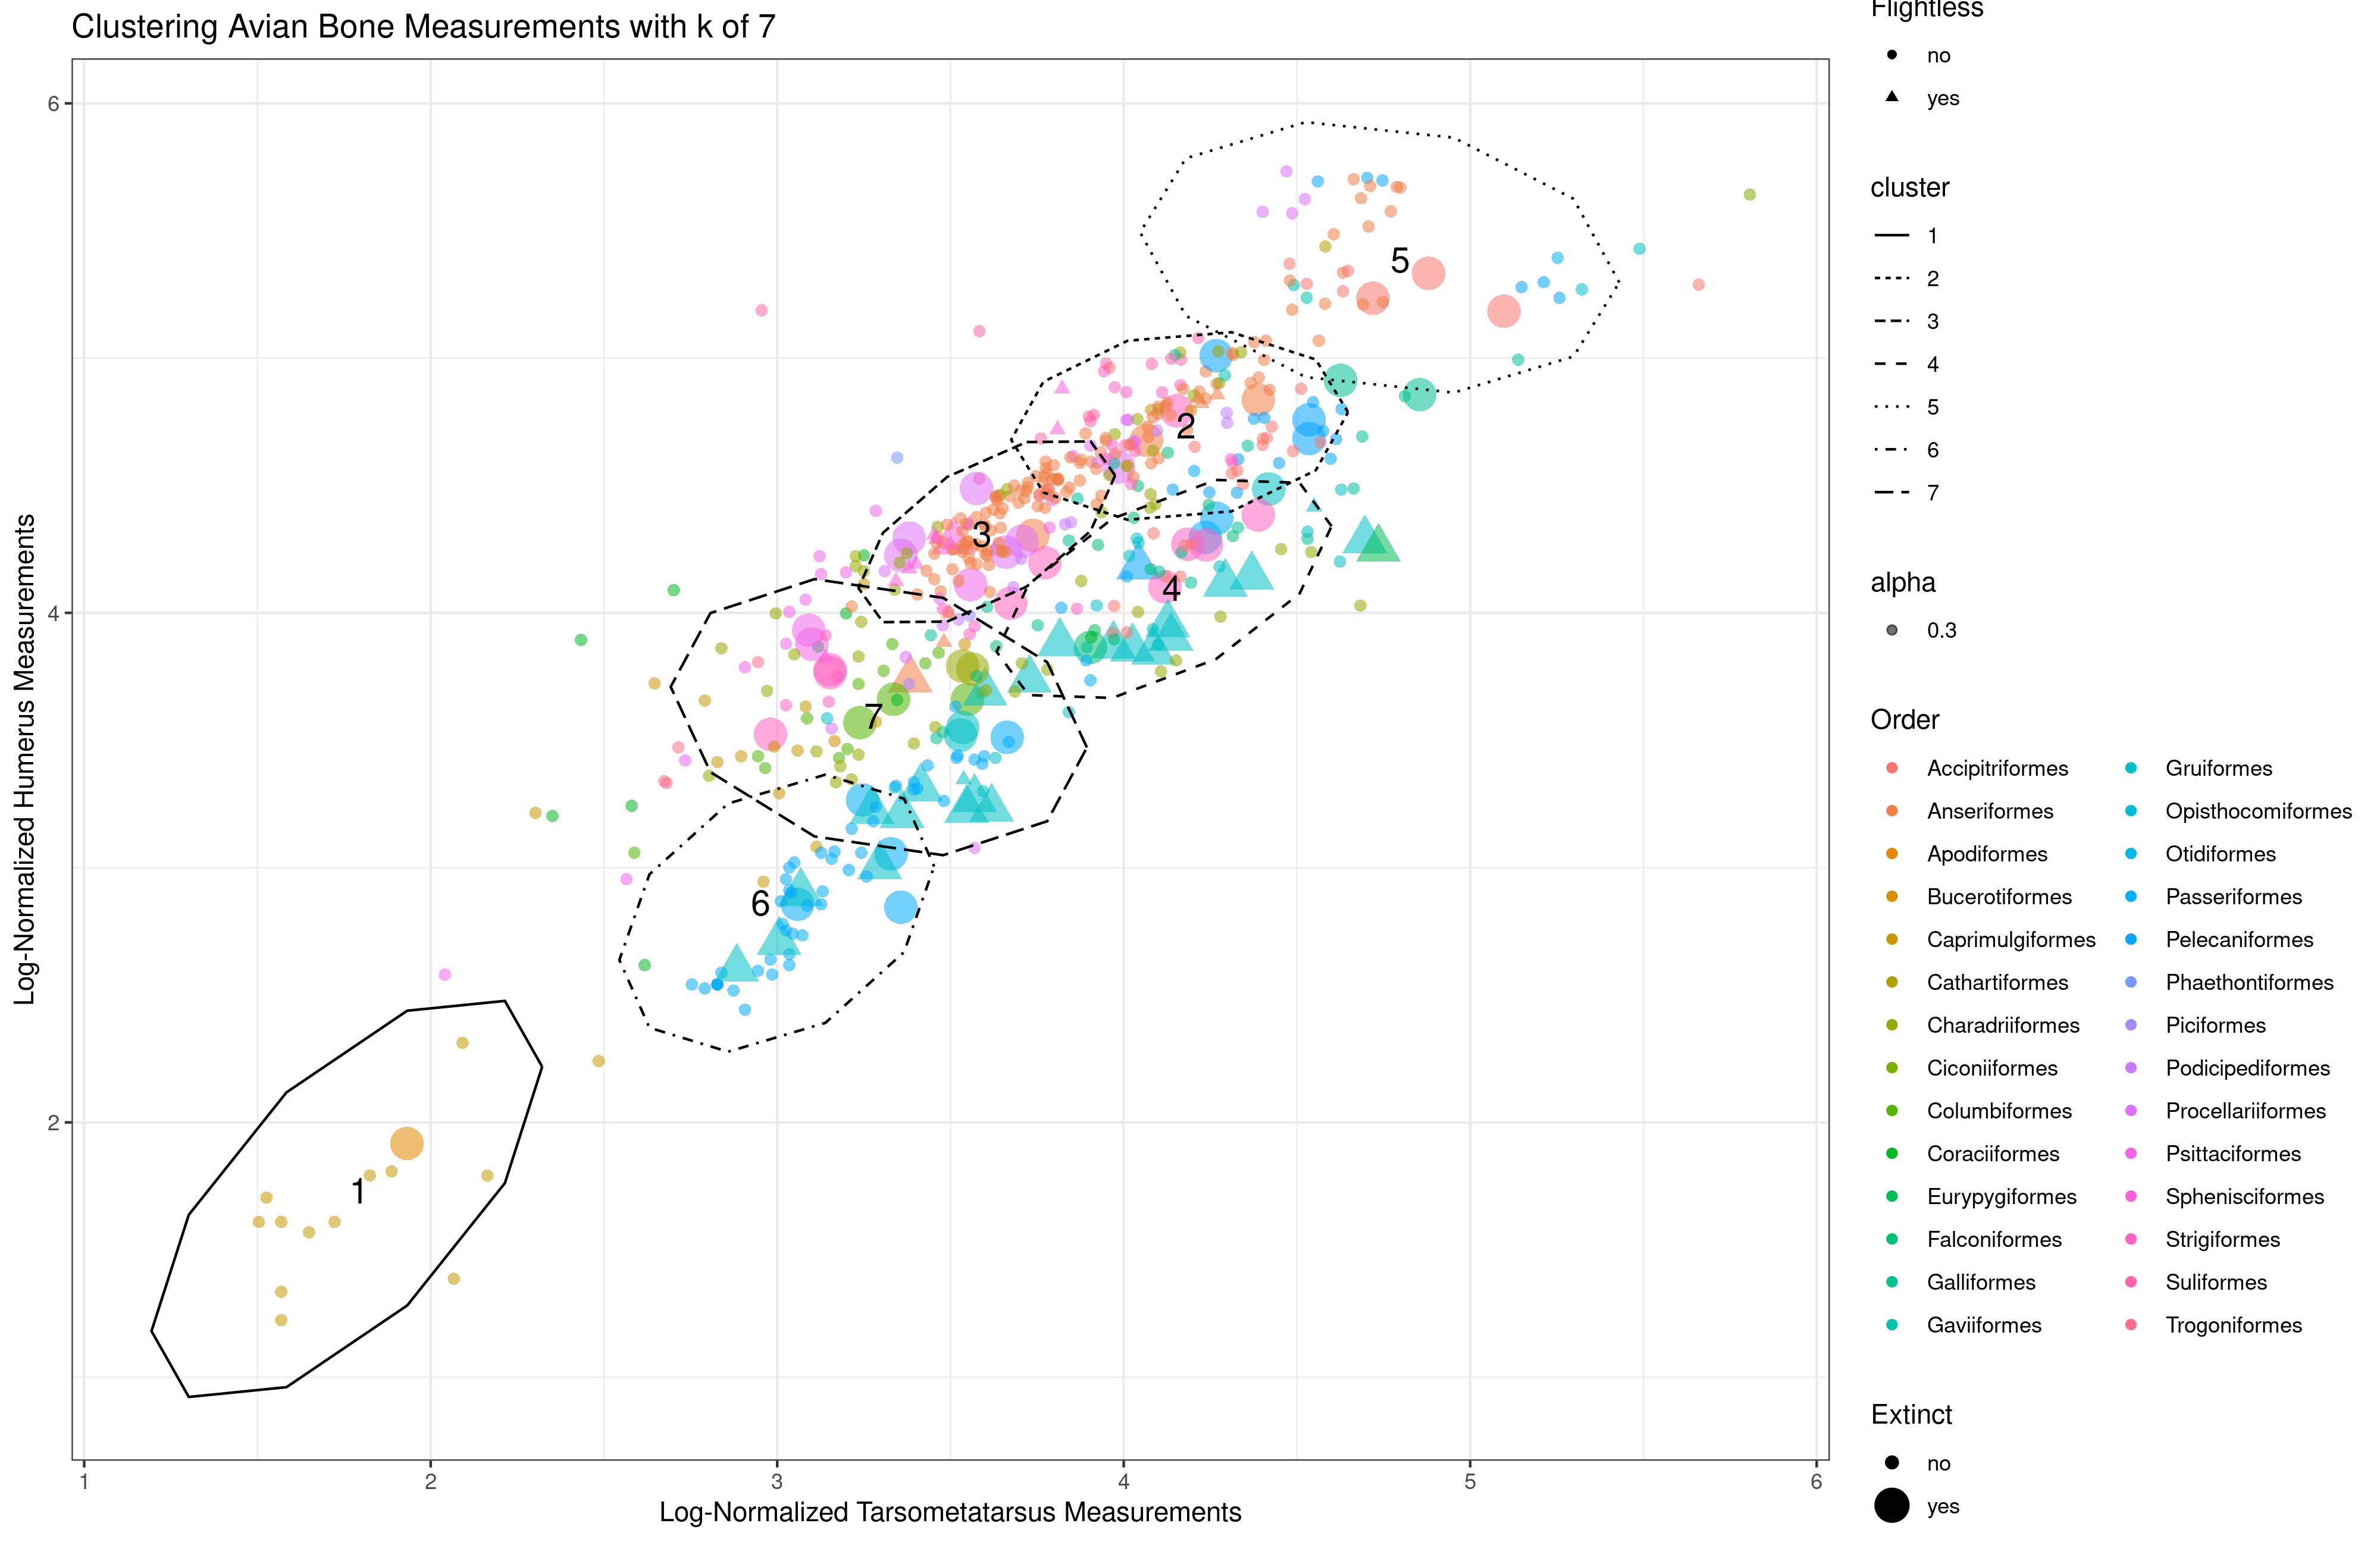
\includegraphics[width=1\linewidth]{../outputs/final_clustered_plot} \caption{Distribution of bird measurements with clusters overlain as ellipses and numbers at cluster centers}\label{fig:figure4}
\end{figure}

\section{Methods}

Body size measurements data was downloaded from data dryad entry
10.5061/dryad.1rn8pk0tb via R script. The groundhog package was used for
package version management and library control. Exploratory data
analysis was carried out using the tidyverse R package \citep{tidy}.
Data was loaded into R using the readxl package, filtered for NA values
using dplyr and coerced using base R \citep{read} \citep{dplyr}.
Variables for k-means clustering were chosen based on availability of
data; the two variables with the most overlapping available values were
chosen for downstream analysis. K-means clustering was performed using
the tidymodels R package \citep{kuhn_tidymodels_2020}. Model variables
were tidied and gathered using the broom R package \citep{broom}. Data
was plotted using ggplot2 \citep{ggplot}.

\section{Discussion}

In the original paper the authors found that birds driven to extinction
by humans were more likely to be larger, flightless, and live on islands
\citep{fromm_big_2021}. In this analysis I aimed to recreate these
findings with an unsupervised learning approach. However, I was unable
to do so. One possible explanation is the data points I used. In my
analysis I filtered much of the data and ended up only using two data
points; Humerus and Tarsometatarsus measurements. Because these two data
points are correlated, it is possible that other relationships in the
data were not able to be elucidated from this specific combination.
Additionally, the authors reached those conclusions by aggregating the
size measurements into a single measurement of estimated body size
\citep{fromm_big_2021}. They estimated bird body size by employing a
linear regression model using data from all the measurements they
gathered to allow for an even comparison between extinct and extant
species \citep{fromm_big_2021}. This esimated body mass metric was then
used in their statistical analysis to compare extinct and extant birds
and how they came to their conclusions. My analysis did not use
estimated body mass, so it is possible that this is the reason I was
unable to come to the same conclusions. In the future, one could attempt
to employ a different unsupervised approach such as a random forest
model using the same estimated body mass measurements to see if that
could recreate their results.

\section{Conclusion}

In this study I aimed to recreate the results of \citet{fromm_big_2021}
using an unsupervised k-means clustering approach but was unable to come
to the same conclusions. Future studies can employ alternative models
using different parts of the data to improve upon my analysis.


% Bibliography
\bibliographystyle{natbib}
\bibliography{bibliography.bib}

\end{document}
